\begin{frame}

\frametitle{Mixture models}
\begin{itemize}
\item A mixture model is a probability distribution with density function, $f$, defined as a linear combination of density functions, $f_1, \dots f_k$, coming from other probability distributions.
\[
f(x, \blue{\pi_1}, \dots, \blue{\pi_k}, \blue{\theta_1}, \dots, \blue{\theta_k}) = \blue{\pi_1} f_1(x, \blue{\theta_1}) + \dots + \blue{\pi_k} f_k(x, \blue{\theta_k})
\]
\item Given a  sample $X$, parameters $\blue{\pi_1}, \dots, \blue{\pi_k}, \blue{\theta_1}, \dots, \blue{\theta_k}$ can be estimated using the $EM$ algorithm.
\item $EM$-algorithm needs the number of components is fixed.
\end{itemize}
\end{frame}

\begin{frame}[t]
\frametitle{Mixture models: Gaussian example}
\begin{block}{Example: fitting a gaussian mixture}
Given a sample $X$ and setting the number of components to $6$. $EM$-algorithm can find the Gaussian mixture which fits ``better'' (with maximum likelihood) to sample $X$.
\end{block}
\medskip
\begin{columns}
\column{0.35\textwidth}%
\only<1>{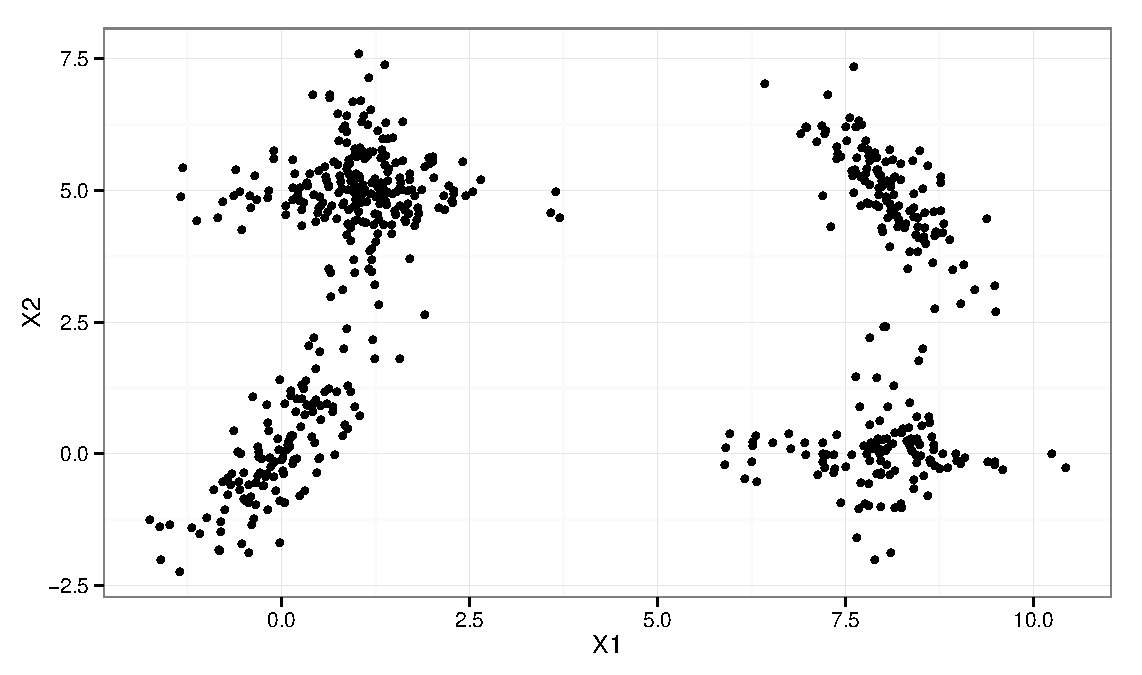
\includegraphics[width=\textwidth]{figures/baudry_ex4_1.pdf}}%
\only<2>{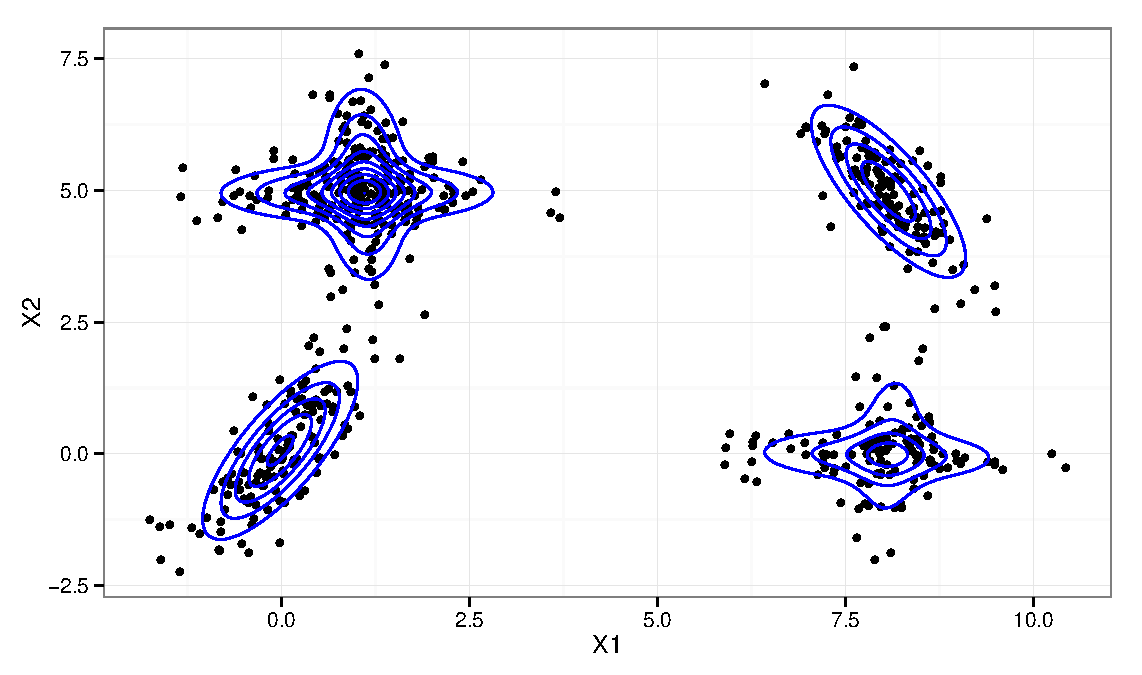
\includegraphics[width=\textwidth]{figures/baudry_ex4_1_contour6.pdf}}

\column{0.6\textwidth}
\uncover<2>{
{\tiny $\pi_1 = 0.12$, $\pi_2 = 0.20$, $\pi_3 = 0.19$, $\pi_4 =0.19$, $\pi_5 = 0.22$, $\pi_6 = 0.08$}

\noindent\rule{4cm}{0.4pt}

{\tiny $\mu_1 = (7.9, -0.02)$, $\mu_2 = (8.07, 4.98)$, $\mu_3 = (1.01, 4.96)$, $\mu_4 = (1.11, 5.12)$, $\mu_5 = (-0.02, 0.06)$, $\mu_6 = (8.10, 0.17)$}

\noindent\rule{4cm}{0.4pt}

{\tiny
$\Sigma_1 = \left(\begin{array}{cc}1.08 & -0.04\\ -0.04 & 0.10 \end{array}\right)$ 
$\Sigma_2 = \left(\begin{array}{cc}0.33 & -0.41\\ -0.41 & 0.85 \end{array}\right)$
$\Sigma_3 = \left(\begin{array}{cc}1.08 & 0.01\\ 0.01 & 0.10 \end{array}\right)$ 
$\Sigma_4 = \left(\begin{array}{cc}0.10 & -0.03\\ -0.03 & 1.08 \end{array}\right)$
$\Sigma_5 = \left(\begin{array}{cc}0.32 & 0.41\\ 0.41 & 0.86 \end{array}\right)$ 
$\Sigma_6 = \left(\begin{array}{cc}0.11 & 0.06\\  0.06 & 1.07 \end{array}\right)$
}
}
\end{columns}
\end{frame}


\begin{frame}
\frametitle{Mixture models: classifying observation}

\begin{itemize}
\item Adjusted density function:
\[
f(x) = \pi_1 \gga{f_1}(x) + \pi_2 \ggb{f_2}(x) + \pi_3 \ggc{f_3}(x) + \pi_4 \ggd{f_4}(x) + \pi_5 \gge{f_5}(x) + \pi_6 \ggf{f_6}(x)
\]
\item Any observation $x_i$ can be classified to component $j$ with maximimum
\begin{eqnarray*} \tau_{ij} &=& \frac{\pi_j f_j(x_i)}{f(x_i) } \end{eqnarray*}
\end{itemize}

\uncover<2->{%
\only<1-2>{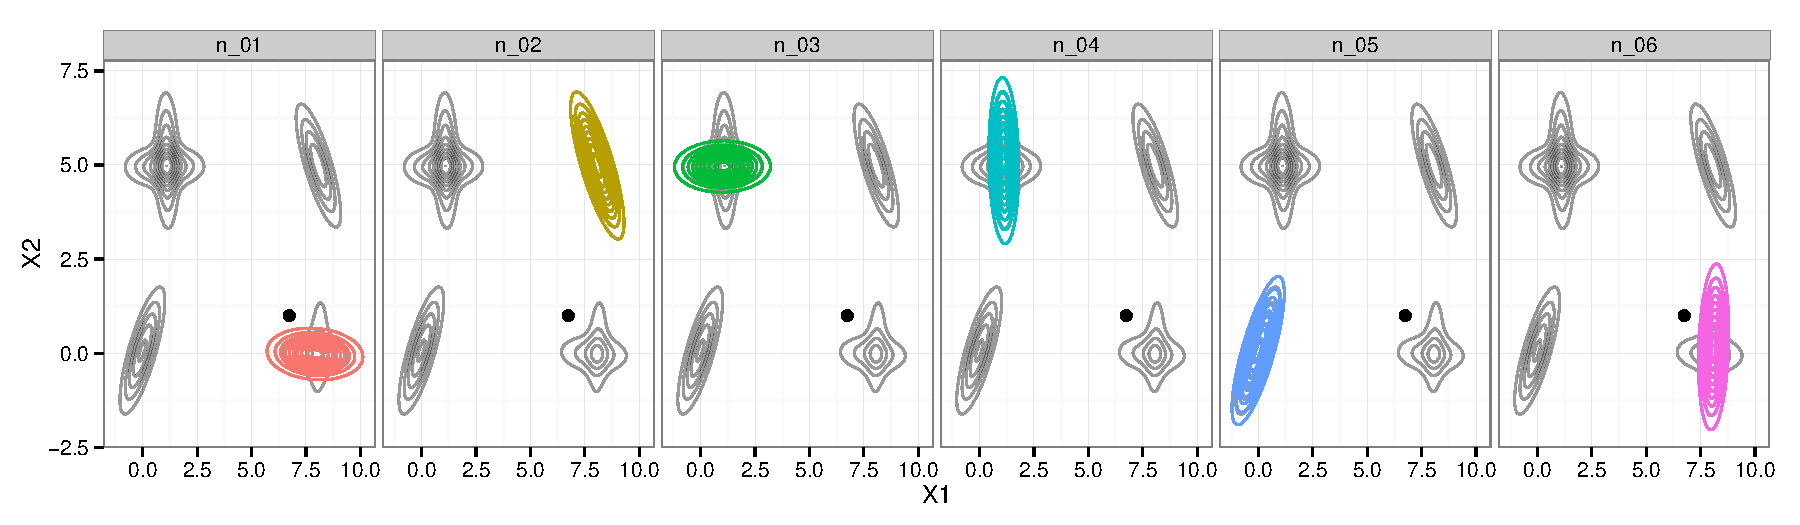
\includegraphics[width=\textwidth]{figures/baudry_ex4_1_all_distributions_one.pdf}}%
\only<3>{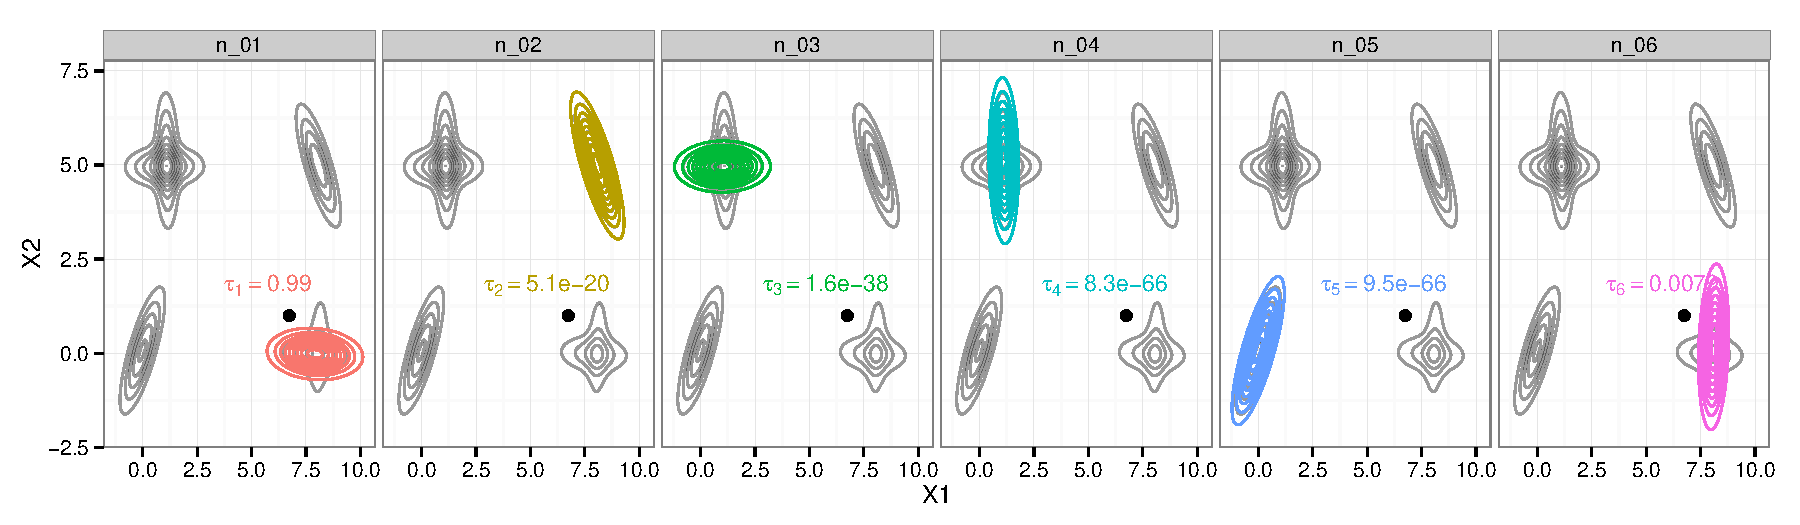
\includegraphics[width=\textwidth]{figures/baudry_ex4_1_all_distributions_one_tau.pdf}}}
\end{frame}

\begin{frame}
\frametitle{Mixture models: merging components}

\begin{columns}[T]
\column{0.4\textwidth}
\centering
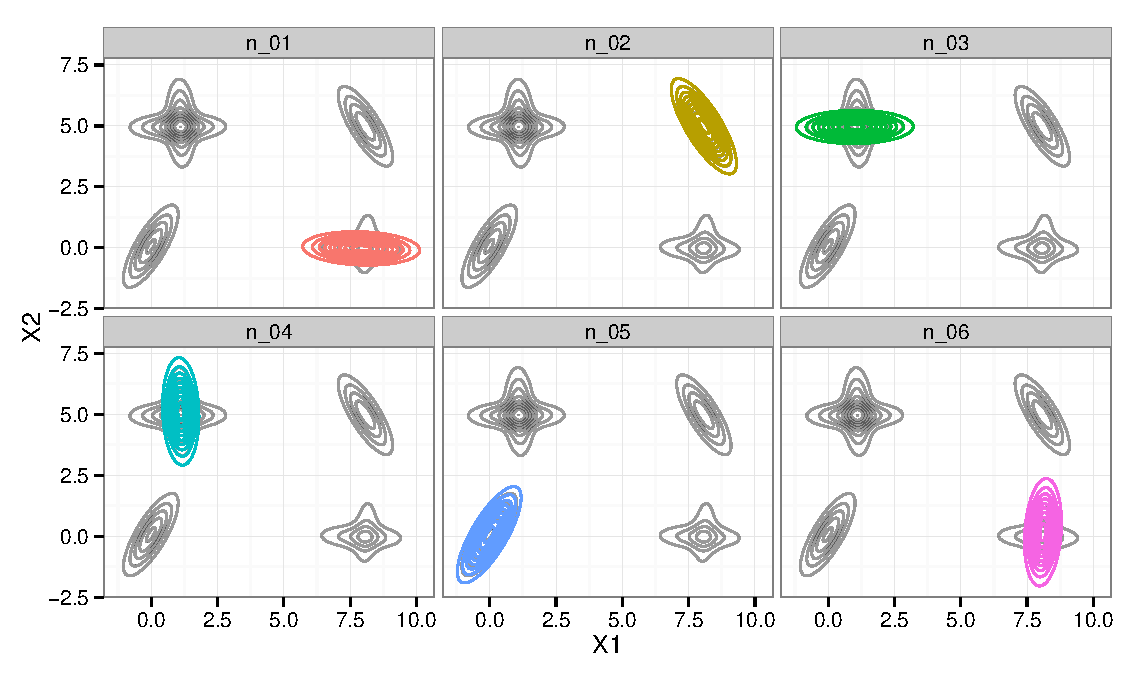
\includegraphics[width=0.9\textwidth]{figures/baudry_ex4_1_all_distributions.pdf}

\bigskip
\uncover<2->{%
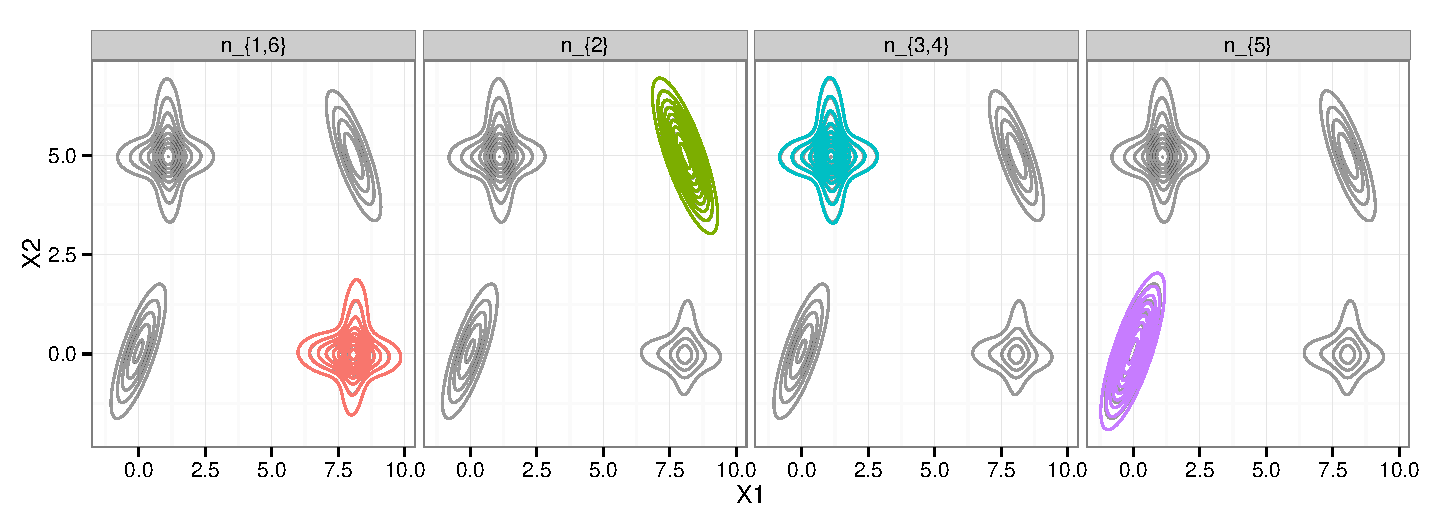
\includegraphics[width=\textwidth]{figures/baudry_ex4_1_all_distributions_4c.pdf}

\uncover<3->{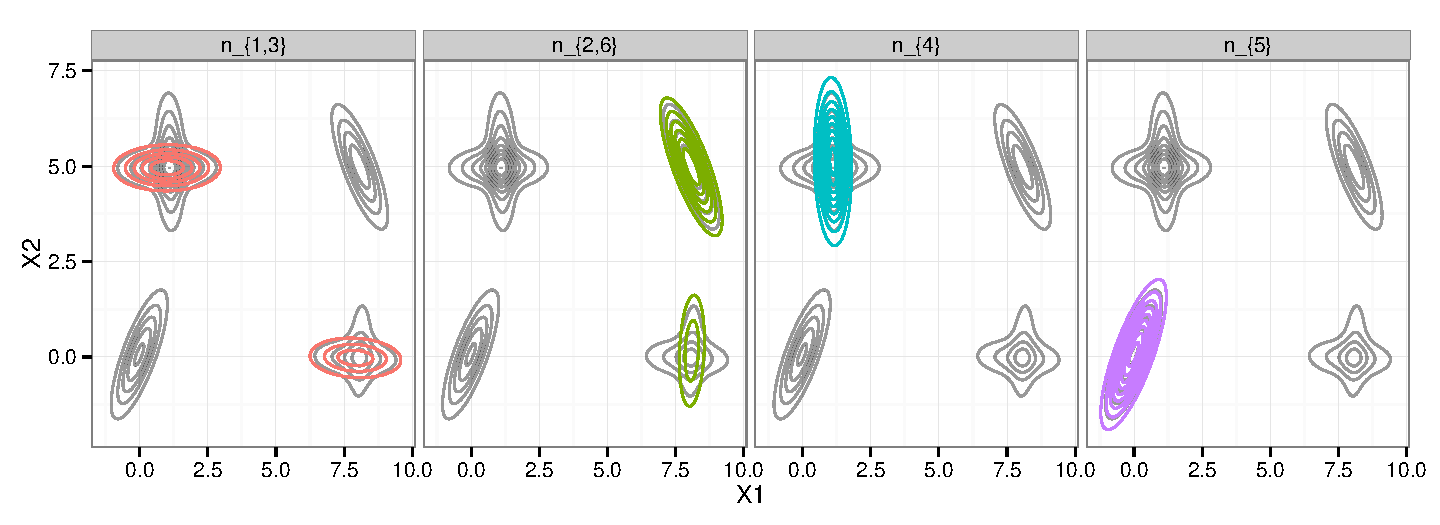
\includegraphics[width=\textwidth]{figures/baudry_ex4_1_all_distributions_4c_b.pdf}}
}

\column{0.6\textwidth}
\small
\begin{itemize}
\item Maybe one cluster is better explained as one mixture of components (``mixture of mixtures'')
\item<2-> From a likelihood point of view it is not possible to choose which ``mixture of mixtures'' is better.
\item<3-> Non-identificability: Both mixtures have the same likelihood.
\item<4> Different authors propose methods to merge components two by two.
\item<4> Here we focus on those methods based on posteriori probabilities which combines the components hierarchically.
\end{itemize}
\end{columns}
\end{frame}

\begin{frame}[t]
\frametitle{Mixture models: hierarchical component merging}
\begin{columns}[T]
\column{0.5\textwidth}
\small
Starting from a mixture model where each component is a cluster

\medskip

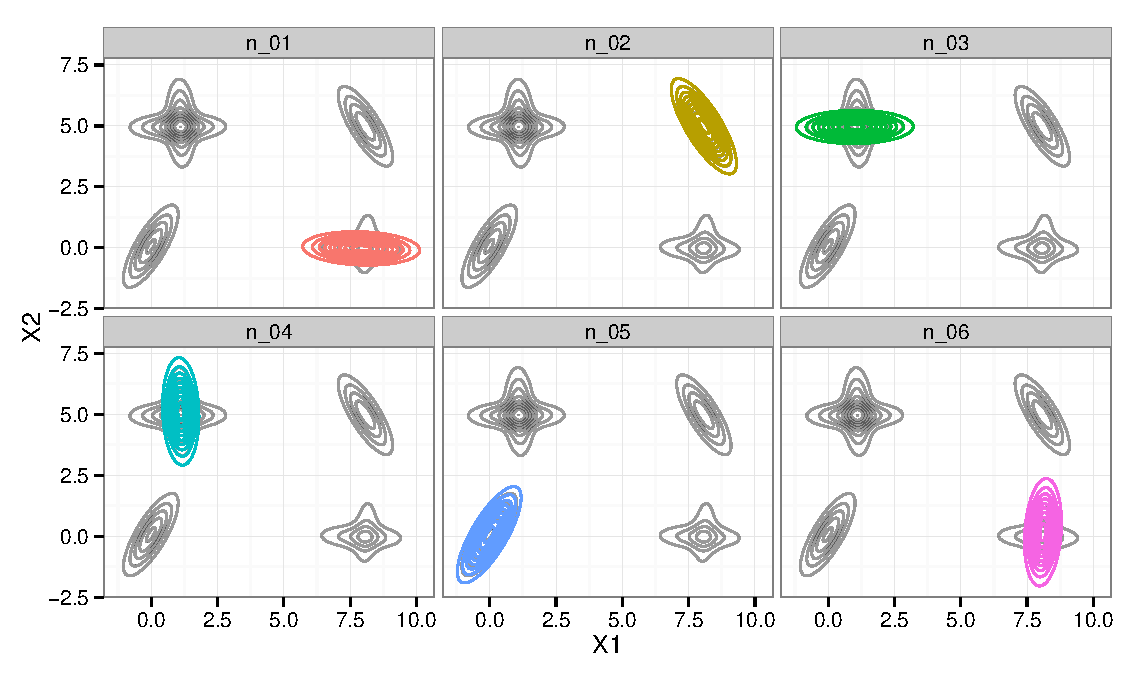
\includegraphics[width=0.9\textwidth]{figures/baudry_ex4_1_all_distributions.pdf}

combine sequentially the components to obtain a hierarchy over the set of components.

\pause
\column{0.5\textwidth}
\centering
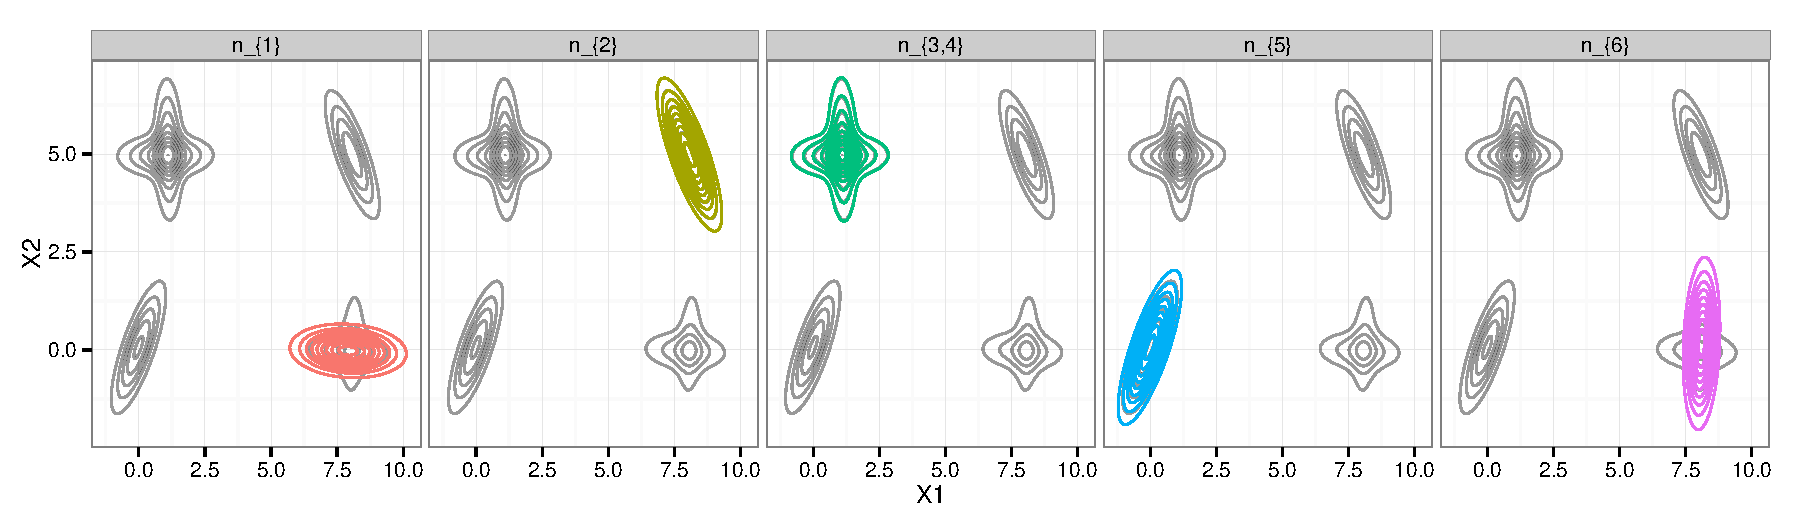
\includegraphics[height=0.2\textheight]{figures/baudry_ex4_1_all_distributions_5c.pdf}

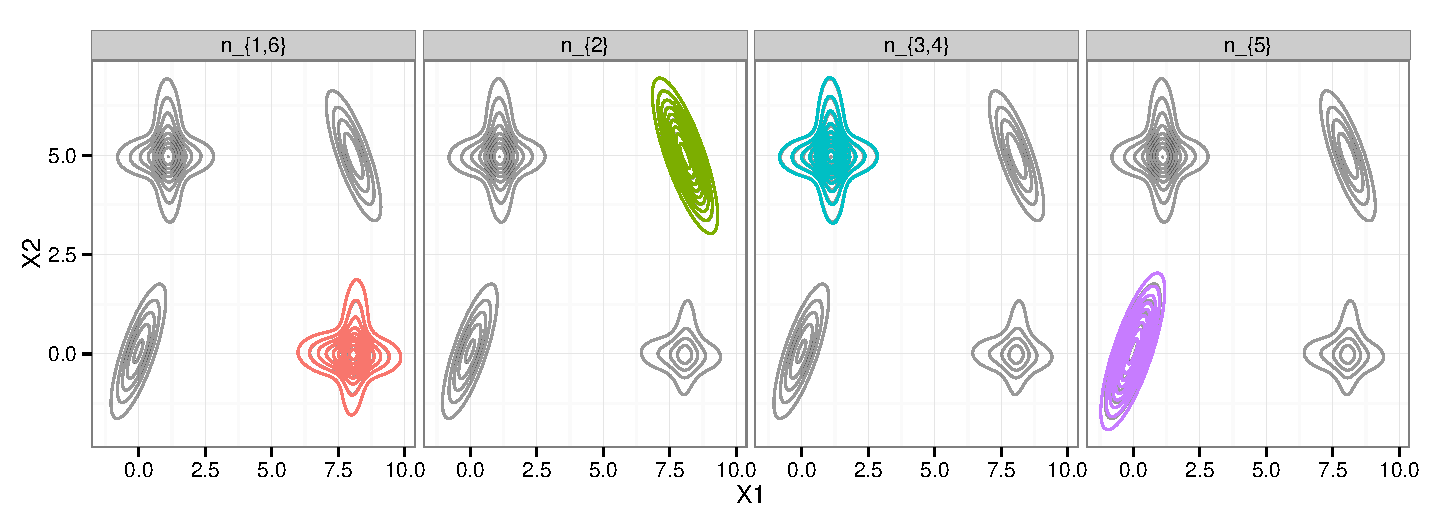
\includegraphics[height=0.2\textheight]{figures/baudry_ex4_1_all_distributions_4c.pdf}

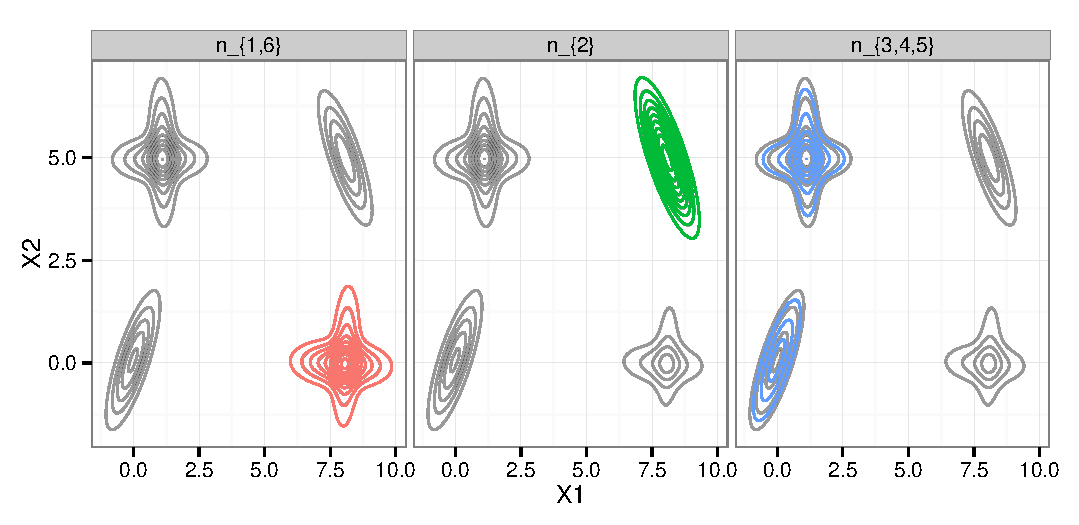
\includegraphics[height=0.2\textheight]{figures/baudry_ex4_1_all_distributions_3c.pdf} 

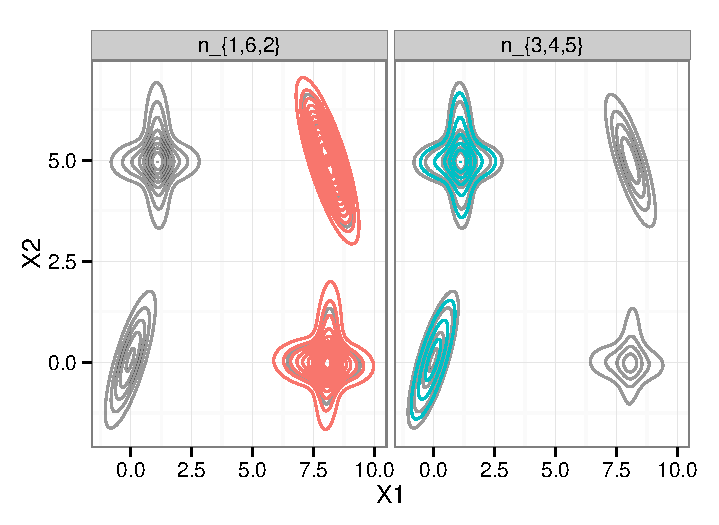
\includegraphics[height=0.2\textheight]{figures/baudry_ex4_1_all_distributions_2c.pdf}
\end{columns}
\end{frame}

\begin{frame}[t]
\frametitle{Our input, our goal: What do we want to do?}

\begin{block}{Input}
A sample of probabilities to belong to each component $C_i$, 
\begin{columns}
\column{0.4\textwidth}
\[ T = \left[ \begin{array}{ccccc}
\idea{(}\tau_{11}\idea{,} & \dots & \tau_{1j}\idea{,} & \dots & \tau_{1k}\idea{),} \\
\vdots      & &    \vdots                     & &    \vdots                     \\
\idea{(}\tau_{i1}\idea{,} & \dots & \tau_{ij}\idea{,} & \dots & \tau_{ik}\idea{),} \\
\vdots      & &      \vdots                   & &       \vdots                  \\
\idea{(}\tau_{n1}\idea{,} & \dots & \tau_{nj}\idea{,} & \dots & \tau_{nk}\idea{)}
\end{array} \right] 
\idea{ \in \mathcal{S}_{[C_1,\dots,C_k]}^k } \]
\column{0.3\textwidth}
\end{columns}
\end{block}

\pause
\begin{alertblock}{Goal}
\alert{Merge} components (sequentially) to obtain a hierarchy over the set of components % $\{C_1, \dots, C_k\}$. %In other words, obtain a binary tree with a set of leafs $\{C_1, \dots, C_k\}$
\end{alertblock}
\end{frame}